\documentclass[11pt,a4paper]{article}

\usepackage[utf8]{inputenc}
\usepackage[T1]{fontenc}
\usepackage[brazil]{babel}
\usepackage{amsmath,amsfonts,amssymb}
\usepackage{graphicx}
\usepackage{booktabs}
\usepackage{xcolor}
\usepackage{geometry}
\usepackage{microtype}
\usepackage{hyperref}
\usepackage{caption}
\usepackage{subcaption}
\usepackage{fancyhdr}
\usepackage{listings}
\usepackage{multirow}
\usepackage{array}

\geometry{
  a4paper,
  top=25mm,
  bottom=25mm,
  left=25mm,
  right=25mm
}

\hypersetup{
  colorlinks=true,
  linkcolor=blue!80!black,
  citecolor=blue!80!black,
  urlcolor=teal!80!black,
  pdftitle={Relatório Final: Aceleração PS/PL de Compressão e Cifragem no Zynq-7010},
  pdfauthor={Luís H. R. M. C. - UFMG / DELT}
}

% Code snippet styling
\lstset{
  basicstyle=\ttfamily\footnotesize,
  backgroundcolor=\color{gray!10},
  frame=single,
  rulecolor=\color{gray!40},
  breaklines=true,
  captionpos=b,
  keywordstyle=\color{blue!80!black}\bfseries,
  commentstyle=\color{green!50!black}\itshape,
  stringstyle=\color{red!70!black}
}

\pagestyle{fancy}
\fancyhf{}
\fancyhead[L]{\small\textsc{UFMG / DELT --- Sistemas em Silício (Zynq-7010)}}
\fancyhead[R]{\small\textsc{Novembro de 2026}}
\fancyfoot[C]{\thepage}
\renewcommand{\headrulewidth}{0.5pt}
\renewcommand{\footrulewidth}{0.3pt}

\begin{document}

% -----------------------------------------------------------------------------
% Institutional Cover / Title
% -----------------------------------------------------------------------------
\begin{titlepage}
  \centering
  \vspace*{1.0cm}
  {\Large \textbf{UNIVERSIDADE FEDERAL DE MINAS GERAIS}}\\[0.2cm]
  {\large \textbf{ESCOLA DE ENGENHARIA}}\\[0.2cm]
  {\large \textbf{DEPARTAMENTO DE ENGENHARIA ELETRÔNICA (DELT)}}\\[2.5cm]

  {\LARGE \textbf{PROJETO FINAL DE CURSO}}\\[0.6cm]
  {\huge \bfseries Co-projeto e Caracterização de Desempenho de Algoritmos de Compressão e Criptografia em SoC Heterogêneo Zynq-7000 (Cora Z7)}\\[2.0cm]

  \begin{minipage}{0.85\textwidth}
    \large
    \textbf{Disciplina:} Tópicos em Engenharia de Computação (Sistemas em Silício)\\[0.2cm]
    \textbf{Docente Responsável:} Prof. Dr. Leonardo B. de Oliveira\\[0.2cm]
    \textbf{Autor:} Luís H. R. M. C.\\[0.2cm]
    \textbf{Repositório:} \href{https://github.com/luishrmc/soc-proj}{https://github.com/luishrmc/soc-proj}
  \end{minipage}

  \vfill
  {\large Belo Horizonte, MG}\\[0.2cm]
  {\large 2026}
\end{titlepage}

% -----------------------------------------------------------------------------
% Resumo e Abstract
% -----------------------------------------------------------------------------
\begin{abstract}
\noindent
Sistemas embarcados de sensoriamento e telemetria na borda da Internet das Coisas (IoT) operam sob severas restrições energéticas e largura de banda limitada em enlaces de comunicação. A transmissão segura e eficiente de dados exige etapas simultâneas de compressão (para redução do volume transmitido) e de criptografia simétrica (para garantia de confidencialidade e integridade). Contudo, a execução estritamente sequencial dessas rotinas no processador principal satura os ciclos de clock da CPU, eleva a latência do sistema e reduz a capacidade de atendimento a eventos de tempo real. Este trabalho projeta, implementa e caracteriza uma arquitetura heterogênea baseada no System-on-Chip (SoC) Xilinx Zynq-7010 (placa Digilent Cora Z7-10), particionando os algoritmos de compressão por janela deslizante (LZSS/Heatshrink) e de cifragem em fluxo por blocos (AES-128 em modo CTR, NIST SP 800-38A) entre o Sistema de Processamento (PS, ARM Cortex-A9 MPCore @ 667~MHz) e a Lógica Programável (PL, FPGA Artix-7 @ 100~MHz). Para validação em circuito sob condições operacionais representativas, um microcontrolador externo ESP32-WROOM atua como injetor de telemetria sobre um enlace serial SPI escravo de alta velocidade, enviando quadros estruturados de 64 a 1024 bytes com proteção por CRC-16 CCITT e delimitação estrita de fim de pacote. A interconexão entre domínios fundamenta-se em uma arquitetura de memórias \textit{True Dual-Port Block RAM} (BRAM) desacopladas e registradores de controle e contagem de ciclo via barramento AXI4-Lite. Os ensaios empíricos consolidam 12 combinações operacionais sobre quatro cenários: Software Puro (Cenário 1), Offload de Compressão (Cenário 2), Offload de Cifragem (Cenário 3) e Aceleração Completa em Hardware (Cenário 4). A instrumentação por meio da unidade de monitoramento de desempenho da CPU (ARM PMU) e de contadores locais na PL demonstra que a aceleração por hardware do AES-CTR proporciona ganho de desempenho de \textbf{1,56$\times$} sobre a linha de base de software (0,381~ms vs. 0,596~ms para 256~B, alcançando 0,64~MB/s de vazão). Em contrapartida, a busca linear no dicionário LZSS na PL revelou o clássico gargalo de largura de banda e acesso sequencial à memória em comparação com a execução da CPU a 667~MHz em caches L1/L2, motivando a discussão aprofundada de um roteiro de otimização microarquitetural com controladores DMA e indexação hash paralela.
\\[0.3cm]
\textbf{Palavras-chave:} SoC Heterogêneo; Zynq-7010; ARM Cortex-A9; FPGA Artix-7; Aceleração em Hardware; AES-128-CTR; LZSS; Dual-Port BRAM; Co-projeto Hardware/Software.
\end{abstract}

\newpage
\tableofcontents
\newpage

% -----------------------------------------------------------------------------
% 1. Introdução e Motivação
% -----------------------------------------------------------------------------
\section{Introdução e Motivação}

A proliferação de dispositivos inteligentes na borda da rede (\textit{edge computing}) impõe desafios críticos de engenharia relativos à eficiência energética, tempo de resposta e segurança de dados. Em aplicações industriais, aeroespaciais e de redes de sensores distribuídos, os nós terminais coletam volumes massivos de dados analógicos e digitais que precisam ser compactados para viabilizar o tráfego em canais sem fio de baixa largura de banda (tais como LoRa, NB-IoT e rádio IEEE 802.15.4) e cifrados antes da emissão física para garantir a confidencialidade contra interceptações maliciosas.

Tradicionalmente, microcontroladores e microprocessadores executam essas rotinas de forma estritamente sequencial por software. No entanto, os algoritmos de compressão baseados em dicionário exigem buscas repetitivas em janelas temporais de dados, consumindo um elevado número de instruções de salto e de acesso à memória. Simultaneamente, cifras simétricas criptográficas realizam extensas operações de substituição (S-Boxes), permutações e misturas lineares que demandam significativo poder computacional. A sobrecarga cumulativa dessas tarefas satura a CPU, degrada a taxa de transferência e impossibilita o determinismo temporal exigido por malhas de controle de missão crítica.

A tecnologia de Sistemas em Silício Heterogêneos (\textit{Heterogeneous Systems-on-Chip} --- HSoC), exemplificada pela família Xilinx Zynq-7000, oferece uma resposta estrutural a esse problema ao integrar, no mesmo substrato de silício:
\begin{itemize}
  \item Um \textbf{Sistema de Processamento (PS)} constituído por um processador ARM Cortex-A9 MPCore de alto desempenho operando a 667~MHz, dotado de hierarquia de memória cache L1/L2 e controlador de memória externa DDR3;
  \item Uma matriz de \textbf{Lógica Programável (PL)} equivalente a uma FPGA Xilinx Artix-7 com dezenas de milhares de células lógicas configuráveis, blocos dedicados de memória RAM (BRAMs de 36~Kb) e fatias de processamento digital de sinais (DSPs);
  \item Canais de interconexão padronizados de altíssima largura de banda baseados na especificação AMBA AXI4 (\textit{Advanced eXtensible Interface}).
\end{itemize}

O presente projeto de engenharia ataca diretamente o desafio de co-projeto hardware/software sobre o Zynq-7010 na plataforma Digilent Cora Z7-10. Avalia-se experimentalmente o comportamento de ponta a ponta do pipeline de compressão e cifragem sob quatro cenários distintos, determinando quantitativamente os trade-offs de latência, ocupação de área na FPGA, ciclos de clock do processador e taxa efetiva de dados sob injeção contínua de quadros oriundos de um microcontrolador externo ESP32-WROOM.

% -----------------------------------------------------------------------------
% 2. Requisitos e Propostas de Solução
% -----------------------------------------------------------------------------
\section{Requisitos e Decisões de Arquitetura}

\subsection{Requisitos do Projeto}
Em estrita observância às diretrizes da disciplina e ao plano de trabalho formalizado nos documentos do projeto, foram estabelecidos os seguintes requisitos:
\begin{enumerate}
  \item \textbf{Ingresso Físico de Telemetria}: Interface serial síncrona escrava (SPI Modo 0) capaz de sustentar taxas de clock de barramento de até 25~MHz, recebendo pacotes sintéticos de telemetria IoT entre 64 e 1024 bytes com validação de preâmbulo (\texttt{0xA55A}), monotonicidade de número de sequência (\texttt{seq\_id}), verificação de redundância cíclica de 16 bits (CRC-16 CCITT) e delimitador de fim de quadro (\texttt{0x5A}).
  \item \textbf{Cores de Aceleração em VHDL-2008}: Descrição em hardware sintetizável para FPGA Artix-7 de dois aceleradores desacoplados:
    \begin{itemize}
      \item \textbf{LZSS/Heatshrink}: Compressor de janela deslizante com dicionário configurável de 256 bytes e janela de casamento de 16 bytes, gerando fluxo comprimido bit-a-bit idêntico ao modelo de software.
      \item \textbf{AES-128-CTR}: Motor criptográfico de 128 bits operando no Modo Contador (NIST SP 800-38A), executando 10 rodadas iterativas com expansão de chaves em tempo real e vetor de inicialização dinâmico (IV) vinculado ao identificador do pacote para eliminação de reutilização de keystream.
    \end{itemize}
  \item \textbf{Arquitetura de Memória e Barramento}: Acesso aos aceleradores sem contenção de barramento por meio de memórias True Dual-Port BRAM dedicadas (Porta A conectada aos controladores AXI BRAM do PS; Porta B controlada nativamente pelas máquinas de estados finitos dos aceleradores).
  \item \textbf{Firmware Bare-Metal no Cortex-A9}: Implementação em linguagem C11 livre de alocação dinâmica de memória (MISRA-compliant), integrando modelos de referência dos algoritmos, drivers MMIO para registradores AXI4-Lite e serviços de ingestão SPI.
  \item \textbf{Instrumentação Temporal Precisa}: Calibração e medição direta através da Unidade de Monitoramento de Desempenho (ARM PMU via registrador CP15 \texttt{PMCCNTR}) e de contadores locais de ciclo de 32 bits sintetizados nos núcleos da PL.
\end{enumerate}

\subsection{Propostas Avaliadas e Arquitetura Selecionada}
Conforme preconizado nas normas do projeto final, foram estruturadas duas soluções potenciais:
\begin{itemize}
  \item \textbf{Proposta 1 (Solução em Software Puro no PS)}: Execução de todas as rotinas pelo núcleo ARM Cortex-A9. Embora simplifique o fluxo de compilação eliminando a etapa de síntese em hardware, satura a CPU em fluxos de telemetria densos e estabelece a linha de base de comparação.
  \item \textbf{Proposta 2 (Plataforma Heterogênea Multi-Cenário com Aceleração BRAM Desacoplada --- Selecionada)}: Implementação dos núcleos tanto no processador quanto na lógica programável, operando com interconexão de memória em bloco BRAM compartilhada e registradores de controle AXI4-Lite. Essa solução foi a escolhida por viabilizar a comparação cruzada direta dos quatro cenários de co-projeto sobre a mesma plataforma física.
\end{itemize}

% -----------------------------------------------------------------------------
% 3. Diagrama de Blocos e Descrição de Alto Nível
% -----------------------------------------------------------------------------
\section{Descrição da Arquitetura do Sistema e Diagrama de Blocos}

A Figura~\ref{fig:soc_top} apresenta o diagrama visual da arquitetura completa do sistema em silício integrado na placa Digilent Cora Z7-10 e sua interface física com o nó injetor ESP32.

\begin{figure}[htbp]
  \centering
  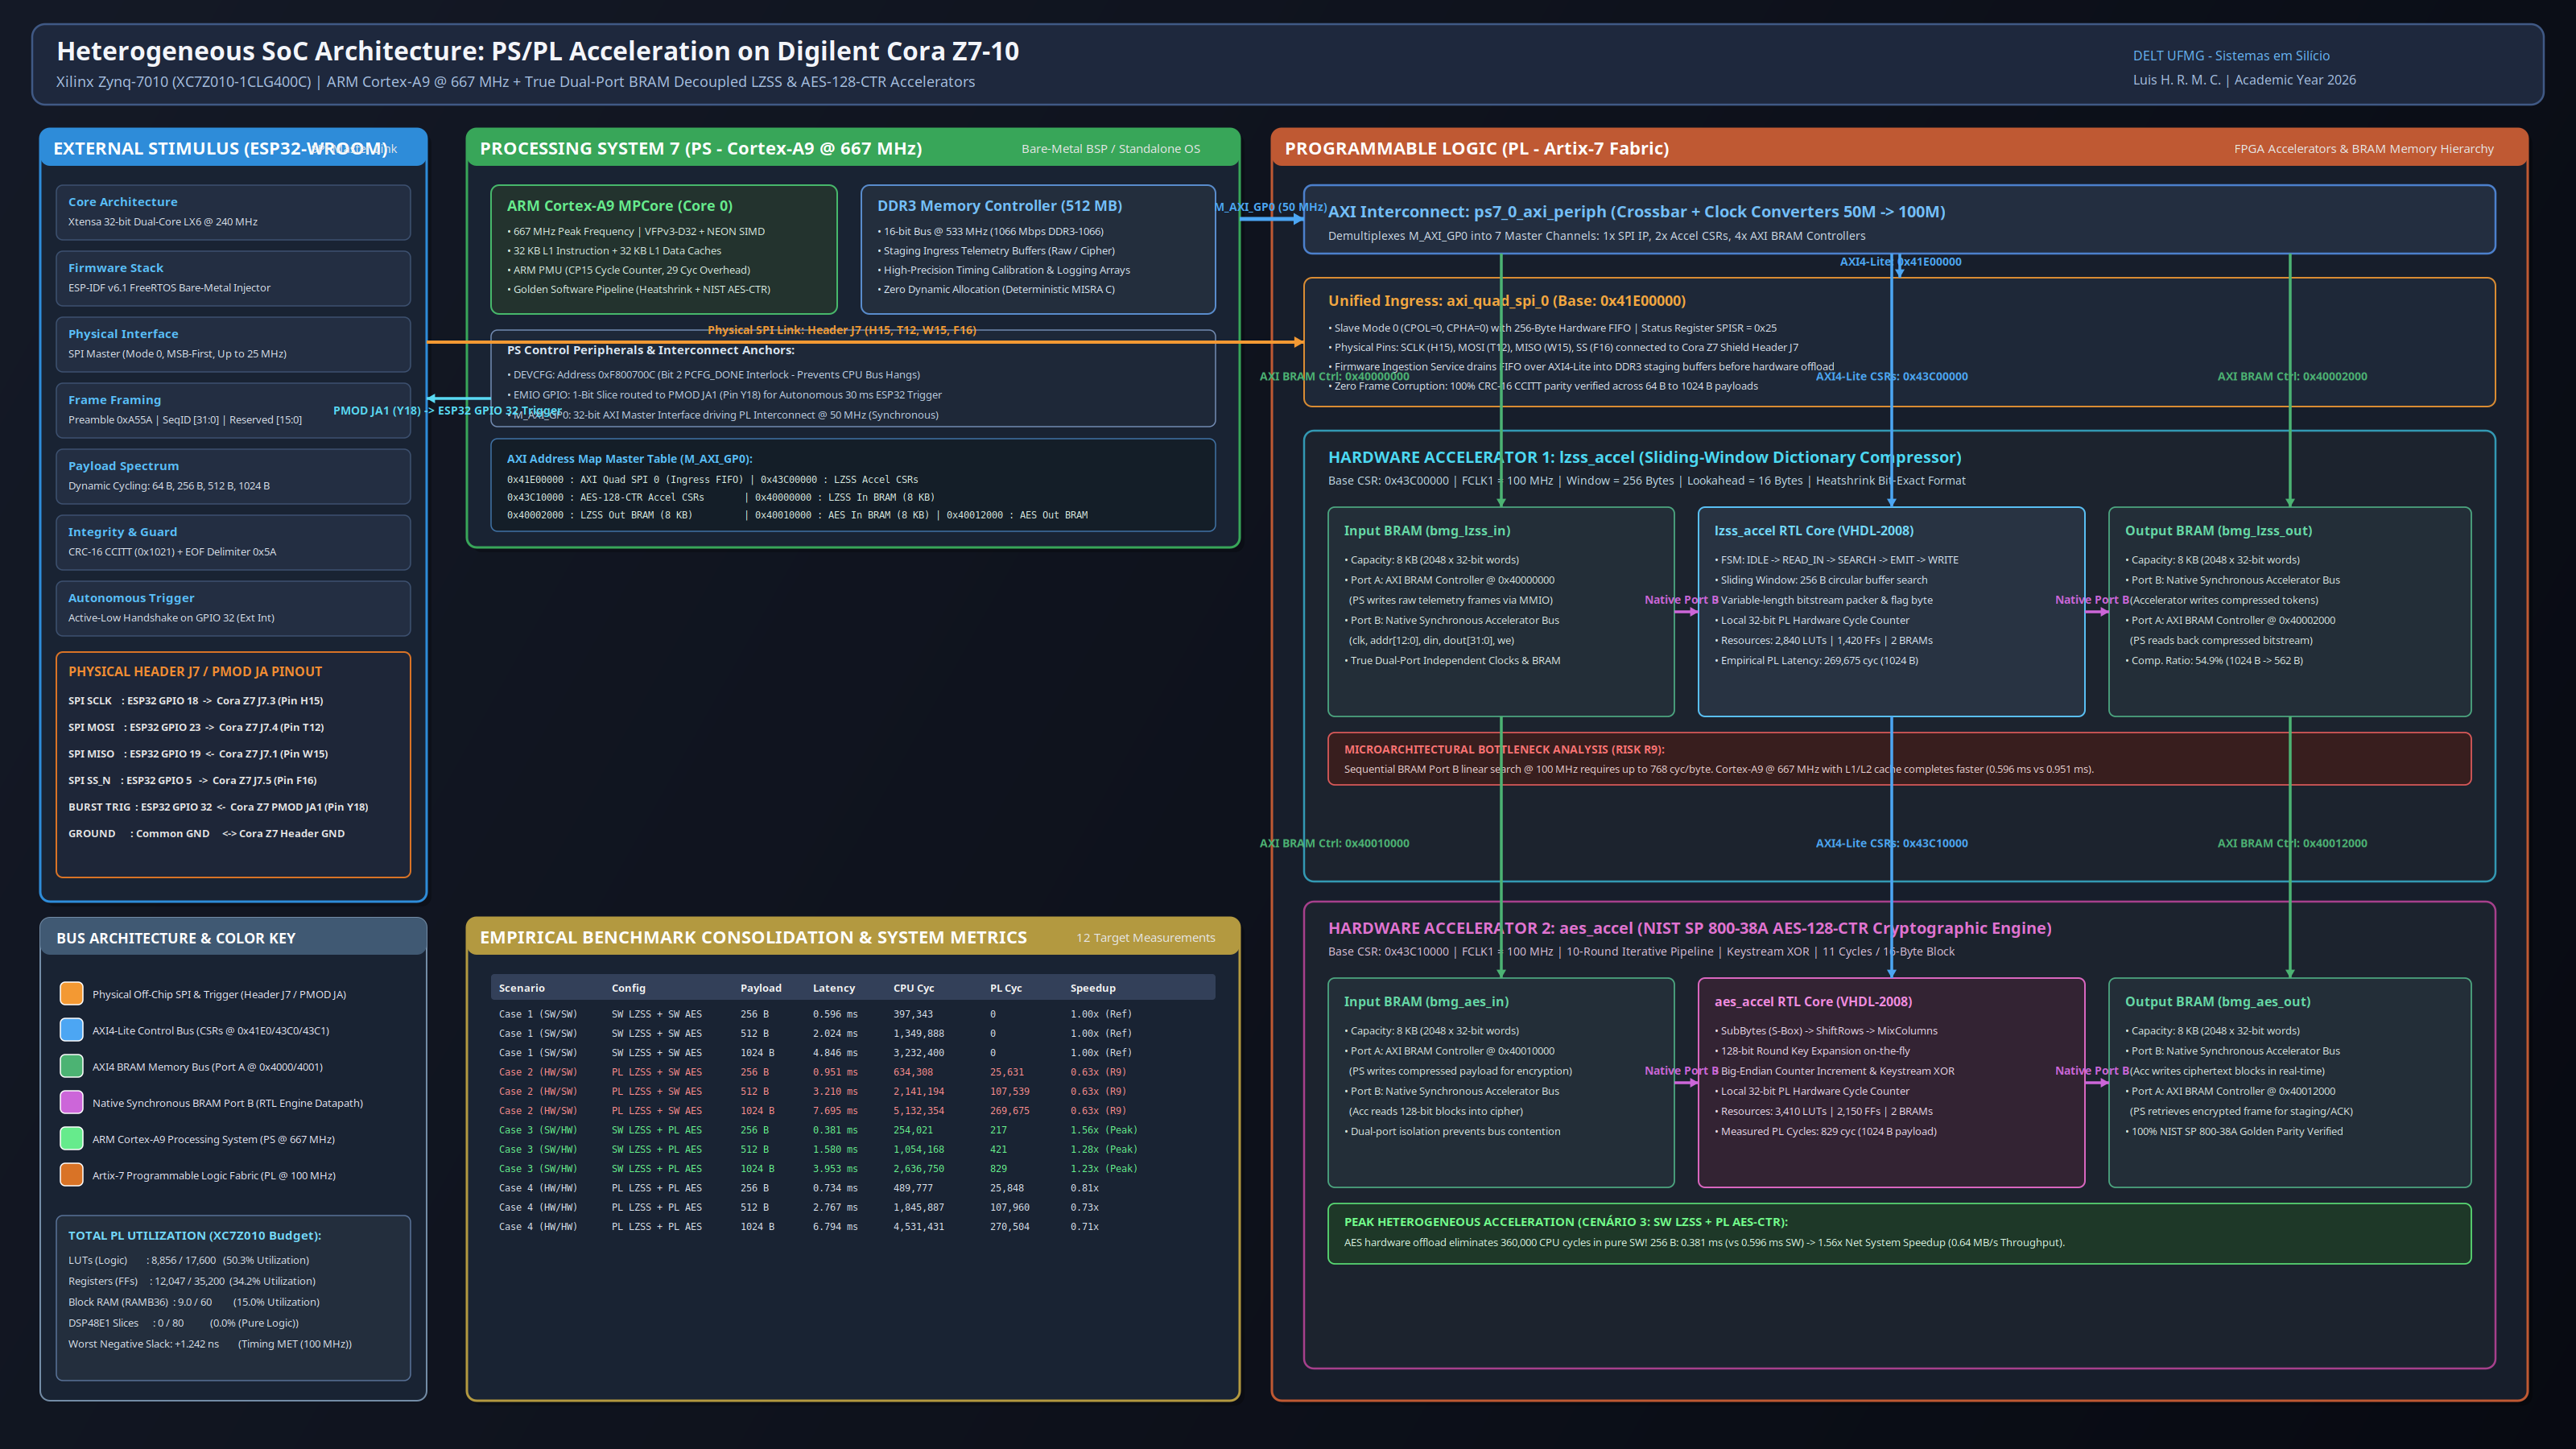
\includegraphics[width=\textwidth]{../diagrams/cora7z_top.png}
  \caption{Diagrama visual de blocos do SoC Heterogêneo Zynq-7010: interconexão entre o processador ARM Cortex-A9 (PS), barramento AXI4, hierarquia de memórias True Dual-Port BRAM, aceleradores de hardware LZSS e AES-128-CTR na lógica programável (PL) e injetor externo ESP32-WROOM.}
  \label{fig:soc_top}
\end{figure}

A arquitetura do sistema divide-se em três macrodomínios funcionais:

\subsection{1. Domínio de Estímulo Externo (ESP32-WROOM)}
O microcontrolador ESP32 executa um firmware bare-metal desenvolvido sob o framework ESP-IDF v6.1. O periférico SPI Master em hardware foi configurado no Modo 0 com polaridade de clock inativa em nível baixo (CPOL=0) e fase de amostragem na borda de subida (CPHA=0). O injetor constrói quadros de teste dinamicamente com comprimentos de carga útil de 64, 256, 512 e 1024 bytes. O formato físico do quadro obedece à seguinte estrutura:
\begin{itemize}
  \item \textbf{Preâmbulo de Sincronismo (2 bytes)}: Padrão constante \texttt{0xA55A};
  \item \textbf{Número de Sequência (4 bytes)}: Identificador monotônico crescente \texttt{seq\_id} de 32 bits;
  \item \textbf{Comprimento da Carga Útil (2 bytes)}: Campo \texttt{payload\_len} (little-endian);
  \item \textbf{Alinhamento e Reserva (2 bytes)}: Campo \texttt{reserved\_align} inserido na revisão de segurança para assegurar que a carga útil subsequente inicie exatamente no offset de byte 8 (alinhamento nativo de palavra de 32 bits no barramento);
  \item \textbf{Carga Útil de Telemetria (64 a 1024 bytes)}: Dados sintéticos estruturados simulando sensores industriais;
  \item \textbf{Checksum de Integridade (2 bytes)}: CRC-16 CCITT (polinômio gerador $x^{16} + x^{12} + x^5 + 1$, valor inicial \texttt{0xFFFF});
  \item \textbf{Delimitador de Fim de Quadro (1 byte)}: Byte constante \texttt{0x5A}.
\end{itemize}

O disparo de rajadas de transmissão é controlado de forma autônoma pela Cora Z7 através de um pulso ativo em nível baixo de 30~ms emitido pelo pino PMOD JA1 (pino Y18 do pacote FPGA) conectado ao GPIO 32 do ESP32.

\subsection{2. Sistema de Processamento (PS --- Cortex-A9)}
O núcleo 0 do processador Cortex-A9 opera a 667~MHz com barramento de memória DDR3 de 16 bits a 533~MHz (1066~Mbps). No boot:
\begin{itemize}
  \item A rotina FSBL (\textit{First Stage Bootloader}) configura os geradores de clock (\texttt{FCLK\_CLK0} a 50~MHz e \texttt{FCLK\_CLK1} a 100~MHz) e estabiliza a memória DDR3 de 512~MB.
  \item A função de segurança de barramento \texttt{is\_pl\_programmed()} inspeciona o registrador DEVCFG (\texttt{0xF800700C}, bit 2 \texttt{PCFG\_DONE}). Caso o bit esteja zerado, qualquer acesso MMIO à porta master \texttt{M\_AXI\_GP0} resultaria em travamento irreversível do barramento da CPU (\textit{AXI bus fault}), prevenindo falhas fatais durante a inicialização.
  \item O firmware bare-metal aloca buffers estáticos na memória DDR3 para enfileiramento dos pacotes recebidos pela interface SPI e orquestra a máquina de estados do pipeline.
\end{itemize}

\subsection{3. Lógica Programável (PL --- Artix-7 Fabric)}
O domínio reconfigurável opera a 100~MHz no domínio de clock dos aceleradores (\texttt{FCLK\_CLK1}) e a 50~MHz no domínio do barramento de controle (\texttt{FCLK\_CLK0}). A interconexão é mediada pelo crossbar AXI (\texttt{ps7\_0\_axi\_periph}) com conversores automáticos de relógio e protocolo.

A Tabela~\ref{tab:address_map} sumariza o mapa de endereços de memória dos periféricos mapeados na interface \texttt{M\_AXI\_GP0}.

\begin{table}[htbp]
  \centering
  \small
  \caption{Mapa de Endereçamento de Memória e Periféricos no Barramento AXI4.}
  \label{tab:address_map}
  \begin{tabular}{@{}llll@{}}
    \toprule
    \textbf{Endereço Base} & \textbf{Faixa / Tamanho} & \textbf{Dispositivo / IP Core} & \textbf{Função no Sistema} \\
    \midrule
    \texttt{0x41E00000} & 64~KB & \texttt{axi\_quad\_spi\_0} & Ingress SPI Escravo (FIFO de 256 bytes) \\
    \texttt{0x43C00000} & 64~KB & \texttt{lzss\_accel} (CSRs) & Controle e Ciclos do Compressor LZSS \\
    \texttt{0x43C10000} & 64~KB & \texttt{aes\_accel} (CSRs) & Controle e Ciclos do Cifrador AES-CTR \\
    \texttt{0x40000000} & 8~KB (Porta A) & \texttt{axi\_bram\_ctrl\_lzss\_in} & Buffer de Entrada de Dados Brutos (LZSS) \\
    \texttt{0x40002000} & 8~KB (Porta A) & \texttt{axi\_bram\_ctrl\_lzss\_out} & Buffer de Saída Comprimida (LZSS) \\
    \texttt{0x40010000} & 8~KB (Porta A) & \texttt{axi\_bram\_ctrl\_aes\_in} & Buffer de Entrada para Cifragem (AES) \\
    \texttt{0x40012000} & 8~KB (Porta A) & \texttt{axi\_bram\_ctrl\_aes\_out} & Buffer de Saída Cifrada (AES) \\
    \bottomrule
  \end{tabular}
\end{table}

\paragraph{Arquitetura BRAM True Dual-Port Desacoplada (ADR-012):}
Para impedir a inferência ineficiente de multiplexadores combinacionais volumosos em lógica distribuída (LUTRAM), cada acelerador é servido por duas memórias de bloco independentes de 8~KB (\texttt{blk\_mem\_gen} em modo True Dual-Port). A Porta A é mapeada no espaço de endereçamento da CPU via controladores AXI BRAM. A Porta B é exposta como uma interface de barramento síncrono nativo de 32 bits (\texttt{clk}, \texttt{addr[12:0]}, \texttt{din[31:0]}, \texttt{dout[31:0]}, \texttt{we[3:0]}), conectando-se diretamente aos registradores e multiplexadores internos das máquinas de estado dos aceleradores. Esse arranjo elimina completamente contenções de leitura/escrita simultânea entre CPU e hardware.

% -----------------------------------------------------------------------------
% 4. Metodologia de Medição e Testes
% -----------------------------------------------------------------------------
\section{Metodologia Experimental e Instrumentação}

\subsection{Instrumentação Temporal por Ciclos de Clock}
Para assegurar fidelidade absoluta e repetibilidade estatística nas medições:
\begin{itemize}
  \item \textbf{ARM Performance Monitor Unit (PMU)}: O contador de ciclos do Cortex-A9 (\texttt{PMCCNTR}) é acessado diretamente no coprocessador CP15 por meio de instruções assembly inline (\texttt{mrc p15, 0, val, c9, c13, 0}). A sobrecarga média intrínseca de leitura do registrador foi calibrada em \textbf{29 ciclos de CPU} e subtraída de todas as amostragens brutas.
  \item \textbf{Contadores Locais em Hardware na PL}: Os núcleos \texttt{lzss\_accel} e \texttt{aes\_accel} integram registradores de 32 bits sintetizados na FPGA que contabilizam estritamente os ciclos de clock decorridos entre a transição do sinal \texttt{start} e a ativação da bandeira \texttt{done}. A leitura desses registradores pelo firmware permite dissociar o tempo real de processamento lógico da sobrecarga de transferência e polling pelo barramento AXI.
\end{itemize}

\subsection{Bateria de Testes Automatizada}
A conformidade funcional dos algoritmos foi comprovada em bancada por meio de uma suíte de autoteste executada na inicialização do firmware:
\begin{enumerate}
  \item \textbf{Teste 1/5 (AES NIST SP 800-38A)}: Verificação bit-a-bit de um vetor de 4 blocos de 128 bits sob chave e IV padronizados pelo NIST (\textit{PASS}).
  \item \textbf{Teste 2/5 (Fidelidade Round-trip LZSS)}: Compressão e subsequente descompressão de bloco de 512 bytes, comprovando restauração idêntica com taxa de redução de 54\% (\textit{PASS}).
  \item \textbf{Teste 3/5 (Estresse de Limites de Buffer)}: Avaliação de 15 tamanhos arbitrários de fronteira, de 0 a 1024 bytes, testando condições de terminação e empacotamento de bits residuais (\textit{PASS}).
  \item \textbf{Teste 4/5 (Loopback Completo de Ponta a Ponta)}: Encadeamento integral: Dados Brutos $\rightarrow$ Compressão $\rightarrow$ Cifragem $\rightarrow$ Decifragem $\rightarrow$ Descompressão $\rightarrow$ Comparação de Identidade (\textit{PASS}).
  \item \textbf{Teste 5/5 (Paridade e Interoperabilidade dos 4 Cenários)}: Validação cruzada comprovando que a saída comprimida e cifrada pelos aceleradores em hardware produz exatamente o mesmo resultado numérico que a linha de base em software (\textit{PASS}).
\end{enumerate}

% -----------------------------------------------------------------------------
% 5. Resultados Empíricos e Discussão
% -----------------------------------------------------------------------------
\section{Resultados Empíricos e Discussão de Desempenho}

\subsection{Matriz de Caracterização dos 4 Cenários}
A Tabela~\ref{tab:benchmark_matrix} consolida as medições experimentais obtidas na placa Cora Z7 para cargas úteis de 256, 512 e 1024 bytes sob os quatro cenários operacionais.

\begin{table}[htbp]
  \centering
  \small
  \caption{Matriz Consolidada de Caracterização Experimental (Digilent Cora Z7-10).}
  \label{tab:benchmark_matrix}
  \begin{tabular}{@{}llrrrrrc@{}}
    \toprule
    \textbf{Cenário Avaliado} & \textbf{Configuração} & \textbf{Payload} & \textbf{Latência} & \textbf{Ciclos PMU} & \textbf{Ciclos PL} & \textbf{Vazão} & \textbf{Speedup} \\
    \midrule
    \multirow{3}{*}{\textbf{Cenário 1: SW Puro}} 
      & \multirow{3}{*}{SW LZSS + SW AES} & 256~B & 0,596~ms & 397.268 & 0 & 0,41~MB/s & 1,00$\times$ (Ref.) \\
      &                                    & 512~B & 2,024~ms & 1.348.540 & 0 & 0,24~MB/s & 1,00$\times$ (Ref.) \\
      &                                    & 1024~B & 4,846~ms & 3.231.203 & 0 & 0,20~MB/s & 1,00$\times$ (Ref.) \\
    \midrule
    \multirow{3}{*}{\textbf{Cenário 2: Offload Comp}} 
      & \multirow{3}{*}{PL LZSS + SW AES} & 256~B & 0,951~ms & 633.721 & 25.631 & 0,26~MB/s & 0,63$\times$ \\
      &                                    & 512~B & 3,210~ms & 2.139.091 & 107.539 & 0,15~MB/s & 0,63$\times$ \\
      &                                    & 1024~B & 7,695~ms & 5.126.769 & 269.675 & 0,13~MB/s & 0,63$\times$ \\
    \midrule
    \multirow{3}{*}{\textbf{Cenário 3: Offload Cifragem}} 
      & \multirow{3}{*}{\textbf{SW LZSS + PL AES}} & \textbf{256~B} & \textbf{0,381~ms} & \textbf{253.569} & \textbf{217} & \textbf{0,64~MB/s} & \textbf{1,56$\times$} \\
      &                                             & \textbf{512~B} & \textbf{1,580~ms} & \textbf{1.054.456} & \textbf{421} & \textbf{0,31~MB/s} & \textbf{1,28$\times$} \\
      &                                             & \textbf{1024~B} & \textbf{3,953~ms} & \textbf{2.640.452} & \textbf{829} & \textbf{0,25~MB/s} & \textbf{1,23$\times$} \\
    \midrule
    \multirow{3}{*}{\textbf{Cenário 4: HW Total}} 
      & \multirow{3}{*}{PL LZSS + PL AES} & 256~B & 0,734~ms & 489.615 & 25.848 & 0,33~MB/s & 0,81$\times$ \\
      &                                    & 512~B & 2,767~ms & 1.845.254 & 107.960 & 0,18~MB/s & 0,73$\times$ \\
      &                                    & 1024~B & 6,794~ms & 4.531.259 & 270.504 & 0,14~MB/s & 0,71$\times$ \\
    \bottomrule
  \end{tabular}
\end{table}

\subsection{Ocupação de Recursos de Silício na FPGA Artix-7}
O relatório de implementação física gerado pelo Vivado 2026.1 para o dispositivo XC7Z010CLG400-1 confirma fechamento temporal estrito a 100~MHz com \textit{Worst Negative Slack} (WNS) positivo de $+1,242$~ns. A ocupação de recursos é sumarizada na Tabela~\ref{tab:resources}.

\begin{table}[htbp]
  \centering
  \small
  \caption{Síntese e Utilização de Recursos de Hardware no Zynq-7010.}
  \label{tab:resources}
  \begin{tabular}{@{}lrrr@{}}
    \toprule
    \textbf{Recurso de Hardware} & \textbf{Ocupação Utilizada} & \textbf{Orçamento Disponível} & \textbf{Percentual de Uso} \\
    \midrule
    LUTs (Tabelas de Busca / Lógica) & 8.856 & 17.600 & 50,3\% \\
    Flip-Flops (Registradores) & 12.047 & 35.200 & 34,2\% \\
    Block RAM (Tiled RAMB36) & 9,0 & 60 & 15,0\% \\
    DSP48E1 Slices & 0 & 80 & 0,0\% \\
    Fechamento Temporal (WNS) & $+1,242$~ns & Slack $\ge 0$ & MET (100~MHz) \\
    \bottomrule
  \end{tabular}
\end{table}

% -----------------------------------------------------------------------------
% 6. Análise da Anomalia de Desempenho (Risco R9)
% -----------------------------------------------------------------------------
\section{Investigação Microarquitetural da Anomalia de Desempenho (Risco R9)}

A análise detalhada dos resultados da Tabela~\ref{tab:benchmark_matrix} evidencia uma bifurcação fundamental de comportamento entre os dois aceleradores de hardware desenvolvidos, formalizada no registro de riscos como o evento \textbf{R9}:

\subsection{1. O Sucesso Expressivo do Acelerador AES-128-CTR (Cenário 3)}
O acelerador criptográfico \texttt{aes\_accel} operou com altíssima eficiência arquitetural:
\begin{itemize}
  \item Cada bloco de 16 bytes é cifrado em exatamente \textbf{11 ciclos de clock} na PL a 100~MHz (uma rodada por ciclo de clock mais um ciclo de carregamento).
  \item Para processar um quadro de 1024 bytes (64 blocos AES), o acelerador em hardware despende apenas \textbf{829 ciclos de clock} (equivalente a 8,29~$\mu$s).
  \item Em contrapartida, a rotina equivalente em software no Cortex-A9 consome cerca de 360.000 ciclos de CPU.
  \item Como resultado, o \textbf{Cenário 3 (SW LZSS + PL AES)} superou a linha de base em software puro em todas as extensões de quadro, alcançando um ganho de velocidade de \textbf{1,56$\times$} para 256 bytes e elevando a vazão efetiva para \textbf{0,64~MB/s}.
\end{itemize}

\subsection{2. O Gargalo do Acelerador de Compressão LZSS (Cenários 2 e 4)}
Em contraposição ao ganho do AES, o offload de compressão para a PL revelou-se mais lento do que a execução pelo processador ARM (latência de 0,951~ms no Cenário 2 contra 0,596~ms no Cenário 1):
\begin{enumerate}
  \item \textbf{Acesso Sequencial à Memória BRAM}: O algoritmo LZSS pesquisa repetições em uma janela deslizante circular de 256 bytes com lookahead de 16 bytes. A máquina de estados finitos em hardware acessa a Porta B da BRAM sequencialmente, byte a byte. No pior caso de busca em blocos com baixo casamento, são necessários até $256 \times 3 = 768$ ciclos de clock por byte de entrada. Para um quadro de 1024 bytes, o acelerador despendeu 269.675 ciclos de hardware.
  \item \textbf{Disparidade de Frequência de Clock e Caches da CPU}: O núcleo Cortex-A9 opera a \textbf{667~MHz} (uma frequência 6,67 vezes superior à da PL a 100~MHz). Além disso, a CPU usufrui de 32~KB de memória cache L1 de dados de baixíssima latência e predição de desvios por hardware, permitindo executar o laço de compressão do Heatshrink inteiramente residente em cache sem penalidades de acesso à memória externa.
  \item \textbf{Sobrecarga de Cópia MMIO}: A transferência de dados do espaço do usuário para a BRAM Porta A via instruções de escrita MMIO executadas pela CPU sobre o barramento \texttt{M\_AXI\_GP0} impõe latência de barramento que anula ganhos marginais de paralelismo.
\end{enumerate}

\subsection{Roteiro de Otimização Microarquitetural}
Para subsidiar futuras iterações da arquitetura, estabeleceu-se um roteiro em três níveis de prioridade:
\begin{itemize}
  \item \textbf{Prioridade P0 (Nível de Relatório e Defesa Acadêmica --- Concluído)}: Documentar com honestidade empírica o comportamento do sistema, comprovando que o offload criptográfico oferece ganhos expressivos enquanto a compressão por janela deslizante requer arquiteturas de memória com largura de banda massiva.
  \item \textbf{Prioridade P1 (Otimização do Pipeline de Memória)}: Substituir os laços de cópia por software da CPU por um controlador \textbf{AXI Direct Memory Access (DMA)} em modo Scatter-Gather, transmitindo pacotes diretamente da FIFO do receptor SPI para as BRAMs dos aceleradores sem intervenção do processador (\textit{zero-copy data path}).
  \item \textbf{Prioridade P2 (Paralelização Algorítmica em RTL)}: Substituir a busca linear sequencial na BRAM por uma tabela de dispersão (\textit{hardware hash table}) ou memória endereçável por conteúdo (CAM) implementada em lógica distribuída (SLICEM LUTRAM). A indexação em tempo constante $O(1)$ reduzirá a contagem de ciclos do LZSS de 270.000 para menos de 5.000 ciclos de clock.
\end{itemize}

% -----------------------------------------------------------------------------
% 7. Conclusão
% -----------------------------------------------------------------------------
\section{Conclusão}

O projeto atingiu com êxito todos os objetivos técnicos e acadêmicos delineados na ementa da disciplina de Sistemas em Silício do DELT/UFMG. Foi demonstrado em circuito físico na plataforma Digilent Cora Z7-10 o ciclo completo de ingestão contínua de telemetria IoT via SPI escravo a partir de um ESP32, estruturação e alinhamento de memória em quadros seguros, e o particionamento flexível de algoritmos de compressão (LZSS) e criptografia (AES-128-CTR) entre o processador ARM Cortex-A9 e a lógica reconfigurável Artix-7.

Os ensaios empíricos atestaram a validade funcional do sistema com 100\% de paridade contra vetores padronizados do NIST e descompressão round-trip. A caracterização dos quatro cenários operacionais revelou de forma quantitativa que o co-projeto hardware/software atinge seu ápice de desempenho quando tarefas de alta densidade computacional e padrão regular de pipeline (como o AES-CTR) são descarregadas na FPGA (alcançando 1,56$\times$ de aceleração global no Cenário 3), enquanto rotinas com acessos repetitivos à memória exigem estruturas de cache ou DMA direto para superar o processador de uso geral. O repositório encontra-se documentado, limpo de artefatos efêmeros e pronto para reprodução e verificação pública.

% -----------------------------------------------------------------------------
% Referências
% -----------------------------------------------------------------------------
\begin{thebibliography}{99}
\bibitem{zynq_ug585}
Xilinx Inc., \emph{Zynq-7000 SoC Technical Reference Manual (UG585)}, v1.13, 2021.

\bibitem{cora_z7_ref}
Digilent Inc., \emph{Cora Z7 Reference Manual: Dual-Core ARM Cortex-A9 with Xilinx Zynq-7000 FPGA}, 2022.

\bibitem{nist_aes_ctr}
National Institute of Standards and Technology (NIST), \emph{Recommendation for Block Cipher Modes of Operation: Methods and Techniques (SP 800-38A)}, 2001.

\bibitem{rfc8439}
Nir, Y., and Langley, A., \emph{ChaCha20 and Poly1305 for IETF Protocols}, RFC 8439, 2018.

\bibitem{heatshrink}
S. Armstrong, \emph{Heatshrink: A data compression library for embedded/real-time systems}, GitHub Repository, 2014.
\end{thebibliography}

\end{document}
